\documentclass[thesis.tex]{subfiles}
\begin{document}
\chapter{Background}

\section{The mobile ecosystem}\label{sec:mobile-ecosystem}

This dissertation talks about the policies surrounding \emph{mobile
ecosystems}; but what, precisely, do we mean by the \emph{mobile
ecosystem}?  Succinctly when we refer to the mobile ecosystem we are
referring to \textbf{the interactions surrounding the use of smart
phones and tablet computers}.  Figure~\ref{fig:mobile-ecosystem} shows
some of the relationships between devices, their users and their
preferences, the stores, companies and all these principal's
policies. Users have phones or other mobile devices.  They may own
personal devices or have a company one.  They may have their own
preferred ways of using the device, or they may be subject to policies
written for their employer.  They download apps, written by developers
from app stores, all with their own policies and some of the stores
may delegate some aspects of their quality control to external vetting
software.  Even just describing these aspects of the mobile ecosystem
\autoref{fig:mobile-ecosystem} is quite complex.

\begin{figure}
  \centering
  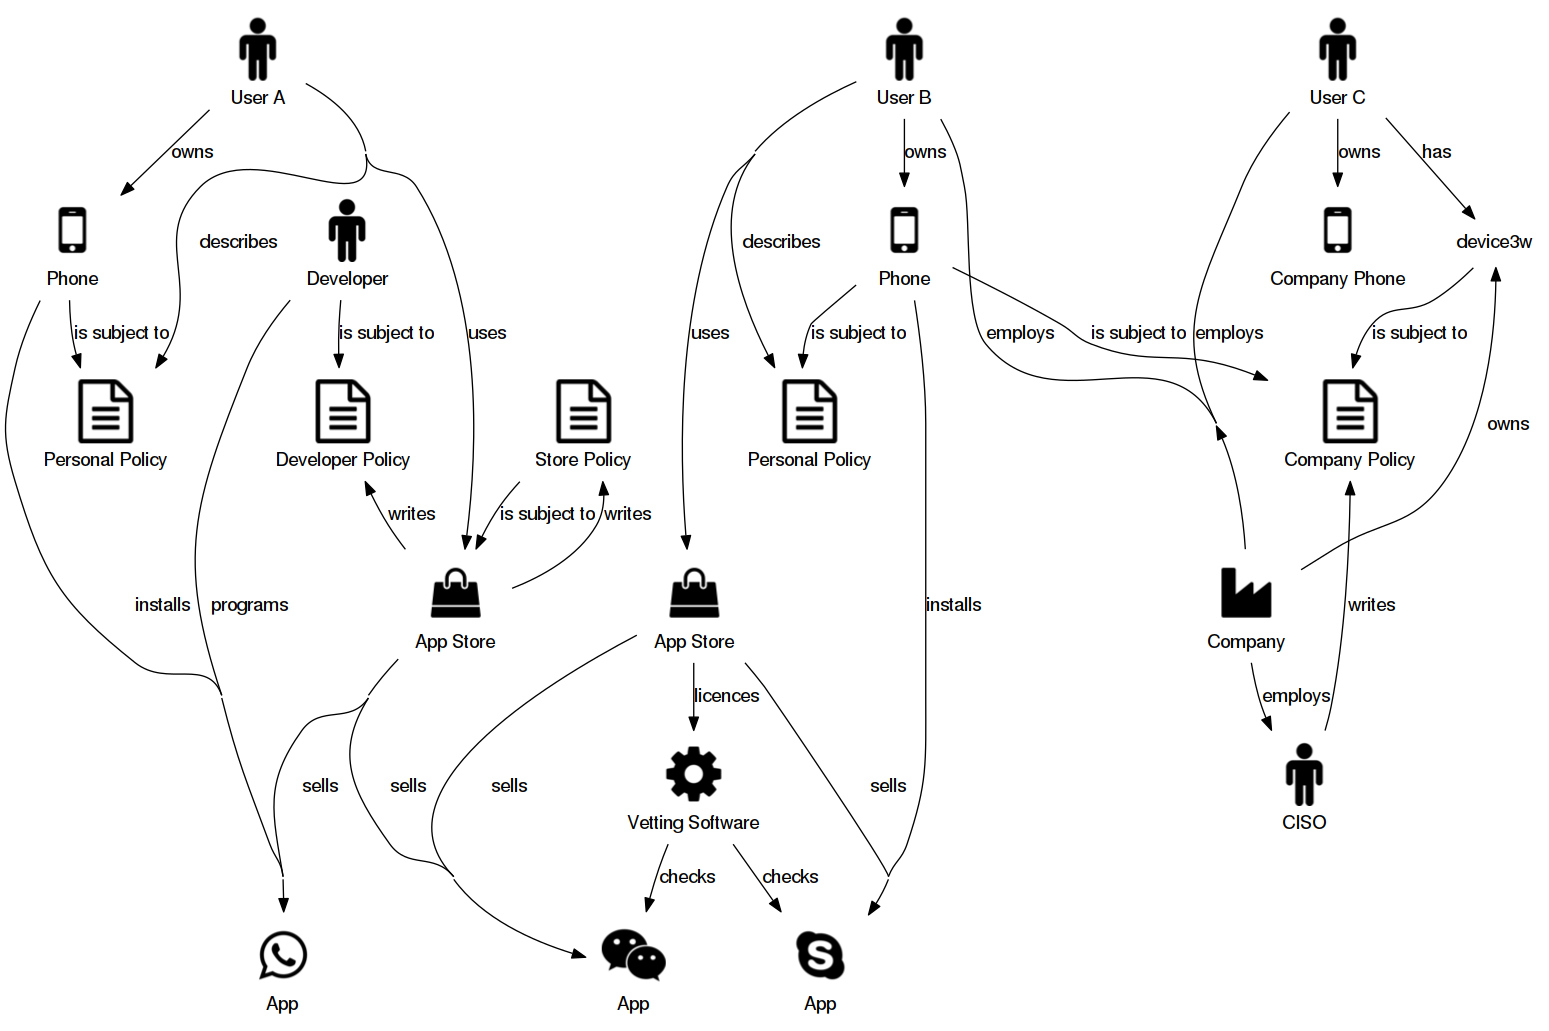
\includegraphics[width=\linewidth]{figures/mobile-ecosystem.png}
  \caption{Interactions between surrounding the use of mobile devices.}
  \label{fig:mobile-ecosystem}
\end{figure}


\subsection{App Stores}

%\todo{Introduce how app stores are the primary mechanism for
%distributing software in the ecosystem.  Describe and possibly show
%the interface, and reviews.  Maybe move the marketshare diagram from
%later on into here?  }

The app store has become the normal method for distributing software
on mobile devices.  These stores run as apps on the device and show
lists of software that the user can install on their devices.  Users
can browse or install free or purchased apps, or read and leave
reviews.  To install an app on an early mobile device the user would
download it on a traditional computer and then transfer it to the
mobile, where they could install it using a package manager.  App
stores considerably streamlined this process, allowing users to find
an install apps straight from their device.  Whilst the app store is
the normal method of installing apps, apps can still be downloaded and
installed manually by side-loading on Android or through iTunes for
iOS.

\begin{figure}
  \centering
  
\includegraphics[width=0.31\textwidth]{figures/store-home.png}
  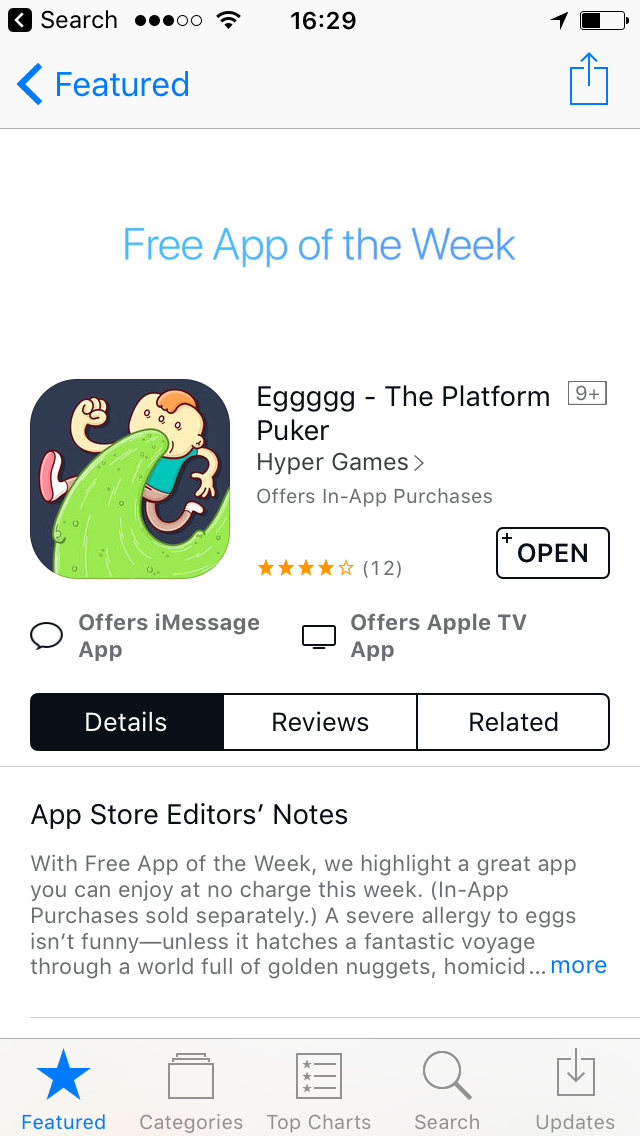
\includegraphics[width=0.31\textwidth]{figures/store-app.png}
  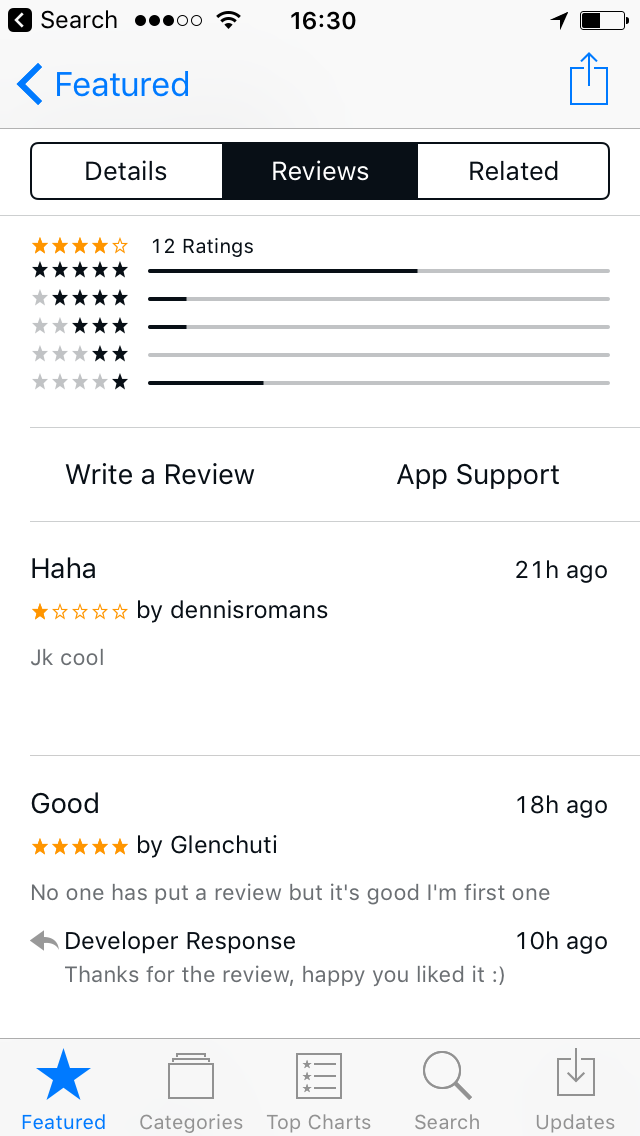
\includegraphics[width=0.31\textwidth]{figures/store-review.png}
  \caption[Apple's App Store.]{Apple's App Store.  Showing the store's frontpage, an app's page, and its reviews.}
  \label{fig:appstore}
\end{figure}

Figure~\ref{fig:appstore} shows Apple's App Store.  Users are first
presented with featured apps, though they can also browse for apps by
category, search, or look at \emph{top charts}.  If a user touches an
app they are presented with more information.  This particular app,
\emph{Eggggg}, is the free app of the week.  The app's name and
age-rating (9+) is shown alongside the a link to the app's developer.
A button is presented for the user to install the app or open it if it
has already been opened.  Additional information is displayed about
the app: it will work with Apple's messaging app, and also with their
Apple TV devices.  The App store editor has, in this case, written a
note about it describing the app which is displayed prominently.  If
the user reads down the page a description of the app by the developer
is also given, as well as screenshots, a changelog, detailed
information including device compatibility, and a link to the apps
privacy policy.  This particular app offers in app purchases and the
user is warned of this prominently on this screen.  A review score is
also displayed. This app has 4 out of 5 stars based on twelve reviews.
If the user touches the review tab, they can see more detailed reviews
by named reviewers.  These can vary in quality (this particular app's
top reviews are not helpful) and the developer can respond to
individual reviews.  User's can optionally write a review for the app.

Whilst Apple and Google's app stores are the largest, others are also
available.  On Android, whilst Google's Play Store is often the
default, users are free to choose other marketplaces if they wish.
One choice is Amazon's Appstore.  It is the default for Amazon's
Kindle Fire tablets, and has special offers for Amazon customers.
Other marketplaces are regional.  In China, where Google web services
cannot be used, alternative markets such as Qihoo360 and Baidu have
sprung up.

Precise numbers of apps in different stores is hard to get, but the
largest stores occassionally give rough
numbers~(\autoref{fig:app-store-apps}).  Google and Apple's stores
have (as of the end of 2016) around 2.5 million apps, with Amazon's
store having considerably less.

\begin{figure}
  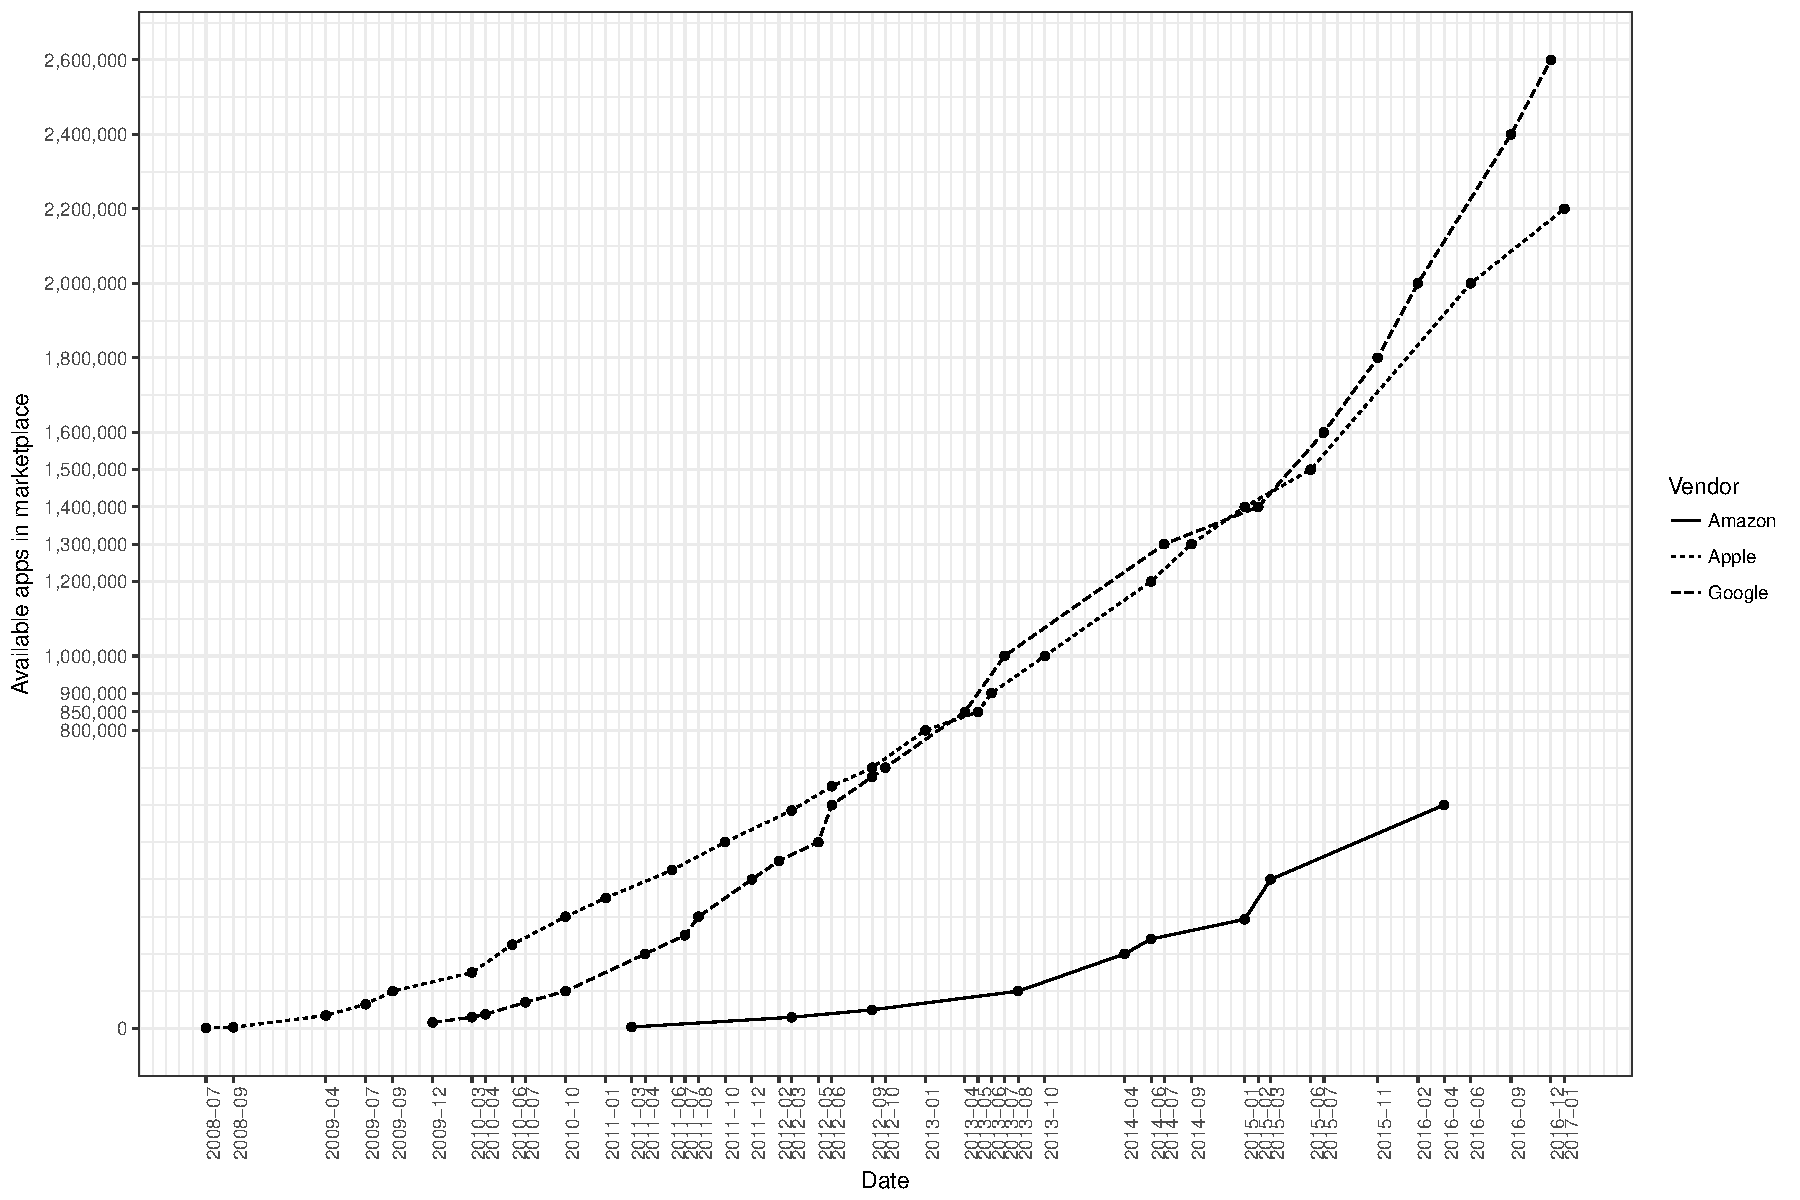
\includegraphics[width=\textwidth]{figures/app-store-apps.pdf}
  \caption[Reported numbers of different apps on various App marketplaces.]{%
    Reported numbers of different apps on various App marketplaces. Data taken from~\cite{statista_google_nodate,statista_apple_nodate,statista_amazon_nodate}.}
  \label{fig:app-store-apps}
\end{figure}

Each of these different stores have different terms and conditions,
and different criteria for developers to sell their apps in.  These
are written in long, dense, legal documents. We will return to these
documents in \autoref{chap:apps-and-stores} when we make a
comparison between them.


\section{SecPAL}

SecPAL is an authorization language developed by Becker~\etal~to
describe policies and delegation chains surrounding distributed
services~\cite{becker_secpal:_2010}. It was designed as a high-level
human-readable language that allowed the policy specification and
maintenance to be separated from the implementation mechanisms.

SecPAL was designed to improve over previous high-level languages in
several areas.  It was designed to be more expressive than
XrML~\cite{kolovski_logic-based_2007},
SPKI/SDSI~\cite{ellison_spki_1999}, and Delegation
Logic~\cite{li_delegation_2003}; and more readable than
XACML~\cite{oasis_extensible_2013} and other XML-based policy
languages.  Furthermore it was designed to be intuitive and
unambiguous with precise semantics unlike other languages (most notably
XACML) which had natural language descriptions with ambiguous and
inconsistent specifications that had been retrofitted to the language
instead of being designed with the language in the first
place~\cite{bryans_reasoning_2005,ramli_logic_2014,masi_formalisation_2012}.

SecPAL's original application was to model and enforce access control
policies in grid computing systems~\cite{becker_secpal:_2010}.  In
this dissertation we describe how the language can be extended to
describe the policies surrounding the mobile ecosystem.

At its core, SecPAL is a language with a simple grammar
(\autoref{fig:secpal-grammar}) and three evaluation rules
(\autoref{fig:secpal-rules}). The language's simplicity makes it easy
to apply to a new domain by instantiating it with predicates and
constraints that describe the domain. This simplicity does not come at
the cost of its expressiveness. SecPAL supports delegation (by using
\emph{can-say} verbs), role and attribute based policies (by using
\emph{can-act-as} verbs) and arbitrary constraints.

\begin{figure}
  \newcommand{\bracetext}[1]{\text{\sffamily #1}}
  \newcommand{\smalltext}[1]{\text{\ttfamily\small #1}}
  \centering
  \begin{equation*}
    \begin{array}{r l}
      \overbrace{\smalltext{`user'}}^{\bracetext{speaker}} &
                                                             \smalltext{ says }\overbrace{\overbrace{\smalltext{ App }}^{\bracetext{subject}}\overbrace{\smalltext{ isRunnable}}^{\bracetext{predicate}}}^{\bracetext{fact}} \\
                                                           & \overbrace{\smalltext{ if App isFree}}^{\bracetext{condition}} \\
                                                           & \overbrace{\smalltext{ where hasPermission(App, `INTERNET') = true}}^{\bracetext{constraint}}.
    \end{array}
  \end{equation*}
  \caption{Structure of a SecPAL assertion.}
  \label{fig:assertion}
\end{figure}

\newcommand{\bnfcomment}[1]{\slshape{\sffamily(#1)}}
\newcommand{\secpal}[1]{\texttt{#1}}
\begin{figure}\footnotesize\centering
  \begin{tabular}{r r l c}
    AC         & $\Coloneqq$ & assertion$_1$ \dots assertion$_n$                      & \bnfcomment{assertion context} \\
    assertion  & $\Coloneqq$ & e \secpal{says} claim.                          \\
    e          & $\Coloneqq$ & \secpal{x}                                       & \bnfcomment{variables}         \\
               & $\vert$     & \secpal{A}                                       & \bnfcomment{constants}         \\
    predicate  & $\Coloneqq$ & \secpal{has} $\vert$ \secpal{can} $\vert$ \dots  & \bnfcomment{predicates}        \\
    D          & $\Coloneqq$ & 0                                                & \bnfcomment{no delegation}     \\
               & $\vert$     & $\infty$                                         & \bnfcomment{unbounded delegation}        \\
    vp         & $\Coloneqq$ & predicate e$_1$ \dots e$_n$                           & \bnfcomment{verb phrase}       \\
               & $\vert$     & \secpal{can-say}$_D$ fact                       \\
               & $\vert$     & \secpal{can-act-as}  e                          \\
    f          & $\Coloneqq$ & e vp                                             & \bnfcomment{fact}              \\
    claim      & $\Coloneqq$ & f \secpal{if} f$_1$,\dots, f$_n$; c             \\
    c          & $\Coloneqq$ & $\top$                                           & \bnfcomment{no constraint}     \\
               & $\vert$     & e$^\prime_1 =$ e$^\prime_2$                      & \bnfcomment{constraints}       \\
               & $\vert$     & \dots                                           \\
    e$^\prime$ & $\Coloneqq$ & e $\vert$ function(e$_1$,\dots e$_n$)           \\
  \end{tabular}
  \caption{BNF description of SecPAL.}
  \label{fig:secpal-grammar}
\end{figure}


\begin{figure}
  \centering
  \begin{eqnarray*}
    \infer[\textsf{\scriptsize cond}]{%
      AC, D \models A\textsf{~says~}fact\theta
    }{%
      \begin{array}[c]{c}
        \left(A\textsf{~says~}\textit{fact}\textsf{~if~}\textit{fact}_1, \ldots, \textit{fact}_k, c\right) \in AC \\
        AC,D\models A\textsf{~says~}\textit{fact}_i\theta \; \forall i \in \{1\cdots k\}
      \end{array}
      & \models{c\theta}
      & \textsf{vars}(\textit{fact}\theta) = \emptyset)
    }\\
    \infer[\textsf{\scriptsize can say}]{%
      AC, \infty \models A\textsf{~says~}\textit{fact}
    }{%
      AC, \infty \models A\textsf{~says~}B\textsf{~can~say}_D \textit{fact}
      & AC, D \models B\textsf{~says~}\textit{fact}
    } \\
    \infer[\textsf{\scriptsize can act as}]{%
      AC, D \models A\textsf{~says~}B~\textit{verbphrase}
    }{%
      AC, D \models A\textsf{~says~}B\textsf{~can~act~as~}C
      & AC, D \models A\textsf{~says~}C~\textit{verbphrase}
    }
  \end{eqnarray*}
  \caption[Inference rules used to evaluate {SecPAL}.]{The inference rules used to evaluate {SecPAL}. All {SecPAL} rules are
  evaluated in the context of a set of other assertions $AC$ as well as an
  allowed level of delegation $D$ which may be $0$ or $\infty$.}
\label{fig:secpal-rules}
\end{figure}

\begin{figure}\centering\sffamily\footnotesize
  \begin{tabular}{c l p{0.6\linewidth}}
    \toprule
    \multirow{3}{*}{\rotatebox{90}{Concepts\hspace{1em}}} & $AC,\theta \vdash q$                     & Defining relation. A query assertion $q$ is valid given the assertions contained in the assertion context $AC$ and a variable substitution $\theta$. \\
    &$\epsilon$                               & The empty substitution. \\
    
    \midrule
    \multirow{5}{*}{\rotatebox{90}{Definitions}} &
    1. $AC,\theta \vdash \overbrace{e \text{ says } fact}^q.$  & if $AC,\infty \models e\theta \text{ says } fact\theta$ and $dom(\theta) \subseteq vars(e \text{ says } fact)$                                       \\
    &2. $AC,\theta_1\theta_2 \vdash q_1, q_2$    & if $AC,\theta_1 \vdash q_1$ and $AC,\theta_2 \vdash_2 q_2\theta_1$                                                                                   \\
    &3. $AC,\theta \vdash q_1 \text{ or } q_2$   & if $AC,\theta \vdash q_1$ or $AC,\theta \vdash q_2$                                                                                                  \\
    &4. $AC,\epsilon \vdash \mathsf{not}(q)$     & if $AC,\epsilon \not\vdash q$ and $vars(q) = \emptyset$                                                                                              \\
    &5. $AC,\epsilon \vdash c$                   & if $\models c$                                                                                                                                       \\
    \bottomrule                             \\
  \end{tabular}
  \caption[SecPAL's semantics.]{SecPAL's semantics as described by Becker~\cite{becker_secpal:_2010}.}
  \label{fig:secpal-semantics}
\end{figure}

SecPAL's semantics are given in \autoref{fig:secpal-semantics}.  A
query $q$ to a SecPAL program (which is a collection of facts and
relationships called the \emph{assertion context} or \emph{AC}) asks
if there exists a renaming $\theta$ such that the rules of SecPAL can
be used to derive the, possibly renamed, query ($AC,\theta \vdash q$
if $AC,\infty \models q\theta$)\footnote{$\vdash$ describes if a query
  is valid with respect to an AC, whereas $\models$ says there is a
  valid proof for a SecPAL using the rules of SecPAL.  Conjugation,
  disjunction and negation are allowed within a query, but not when
  evaluating SecPAL.}.  The renaming must be specific and talk only of
the variables contained in the query, conjunction and disjunction work
as expected.  Negation is only allowed in an extremely limited form: a
query can be not true if it contains no variables and there is no way
to show that the AC supports the query.  This limited form means that
queries remain decidable: the rules inside the AC are not permitted to
use negation.

SecPAL was later extended to add universal quantification, and the
possibility of dynamic assertion retrieval (they defined a safety
condition, but didn't describe a protocol for retrieving assertions).
They also abandoned the roles to use exclusively depth bounded
delegation (citing a lack of uses in
practice)~\cite{moritz_y_becker_secpal:_2009}.  These ideas would be
expanded to create a new language called
DKAL~\cite{gurevich_dkal:_2008}.  Gruevich~\etal~showed how SecPAL
policies could be translated into DKAL
policies~\cite{gurevich_dkal:_2008} so any SecPAL-based policies could
be updated to DKAL.  We don't use these additional features in this
thesis as we did not need the additional expressiveness they provide
to adequately describe the policies in the mobile ecosystem.

\subsection{Delegation in SecPAL}

A key feature of SecPAL is the ability to delegate statements. SecPAL was
designed to make access control decisions over large networks. Rather than have
a centralized decision server where all decisions are made, SecPAL allows
information to be shared through assertions signed by their speaker. This allows
different principals to be responsible for different decisions and make
decisions independently. An example of this, expanded from one given by
Becker~\cite{becker_secpal:_2010}, is of a researcher attempting to run a query
on a cluster, using data from a fileserver (\autoref{fig:delegation-example}).

\begin{figure}
  \centering
  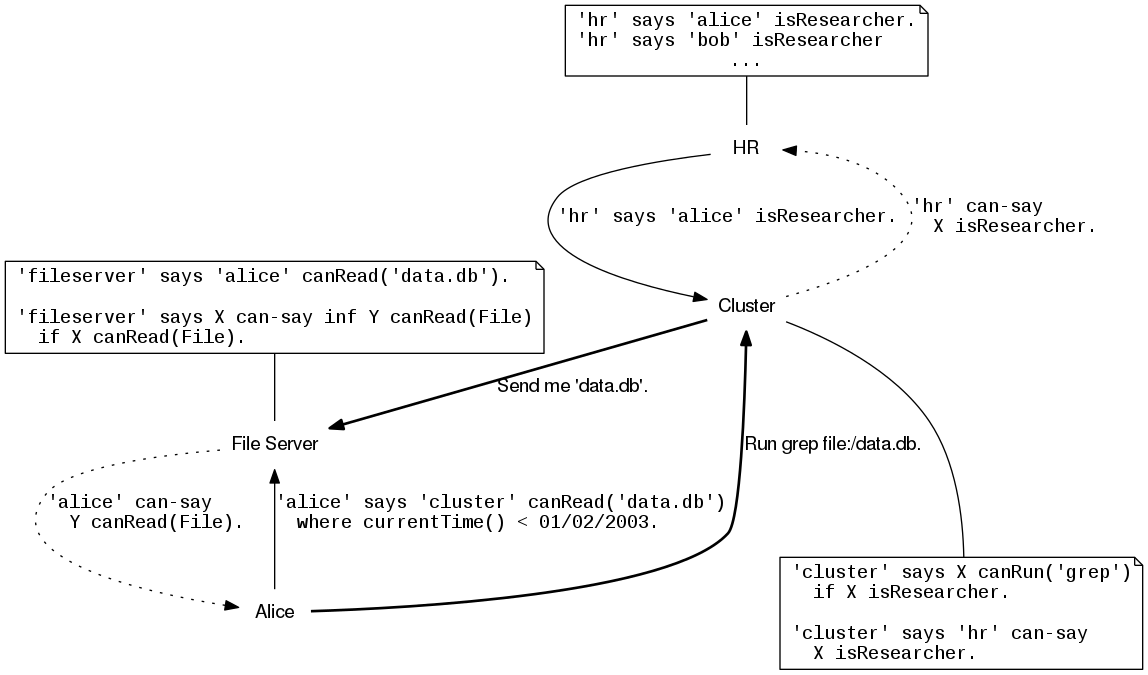
\includegraphics[width=\textwidth]{figures/secpal-example.png}
  \caption[Example of delegation on a cluster.]{Example of delegation when running a command on a cluster.  Bold links show requests, plain links show the sending of SecPAL statements, and dotted links indicate delegation relationships.  SecPAL assertions at each location are shown in notes.}
  \label{fig:delegation-example}
\end{figure}

Alice sends a request to the cluster to run a search on her data on the file-server.
The cluster has a SecPAL policy that only researchers can run the search:
\begin{lstlisting}
'cluster' says X canRun('grep')
  if X isResearcher.
\end{lstlisting}
and a rule that says only HR can say who is a researcher or not.
\begin{lstlisting}
'cluster says 'hr' can-say
  X isResearcher.
\end{lstlisting}
The cluster queries HR if Alice is a researcher or not and HR responds by sending the assertion that she is.
\begin{lstlisting}
'hr' says 'alice' isResearcher.
\end{lstlisting}
The cluster does not know how HR knows that Alice is a researcher, but
is content with HR's assertion that she is.  HR may have a SecPAL
instance and policy of their own to make this and send it to the
cluster, or they might be using a conventional database.  Provided
they give this signed SecPAL assertion to the cluster, it doesn't care
how they came by it.  The one limitation the cluster has is that it
\emph{must} be HR who tells them; HR cannot delegate the decision
further.

With the cluster convinced that Alice is authorized to run the search,
the cluster requests the database from the file server.  The file
server knows that Alice can read her data and that anyone who can read
a file is permitted to say who else can read it.
\begin{lstlisting}
'fileserver' says 'alice' canRead('data.db').
'fileserver' says X can-say inf Y canRead(File)
  if X canRead(File).
\end{lstlisting}
Using SecPAL, the file server, determines that Alice can say who can
read her data.  Alice provides the file server with a statement that
the cluster is authorized to read her file (for a short time
period).
\begin{lstlisting}
'alice says 'cluster' canRead('data.db')
  where currentTime() < 01/02/2003.
\end{lstlisting}
Dutifully the file server provides the cluster with the data
it required.  The cluster runs the search and hands the results back to Alice.

\begin{figure}
  \centering
  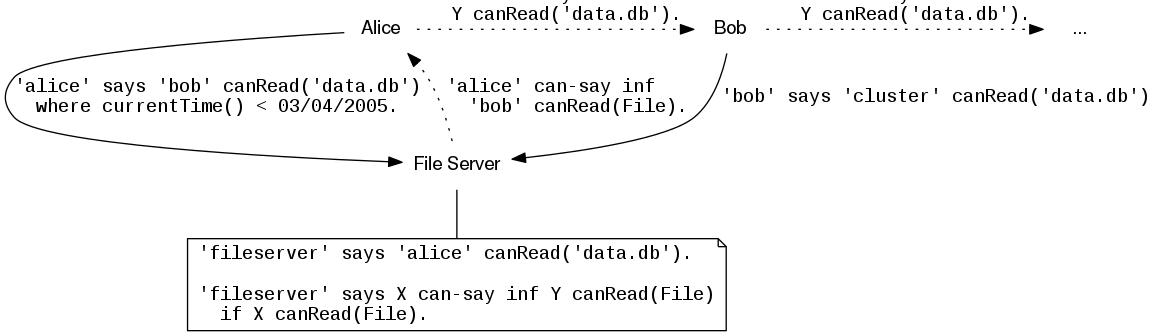
\includegraphics[width=\textwidth]{figures/secpal-example-delegation.png}
  \caption{Example of unbounded delegation.}
  \label{fig:unbounded-example}
\end{figure}

This simple example shows how different principals can make decisions using delegation mechanisms, and by sharing assertions.
SecPAL allows for more complicated delegation relationships, however. When checking who could access Alice's data, the file server allowed Alice the ability to delegate the decision of who could read her file by using the \texttt{can-say inf} verb.
Alice might allow Bob to share her data set with others who might also be allowed to share it for a limited time (\autoref{fig:unbounded-example}).

\begin{figure}
  \centering
  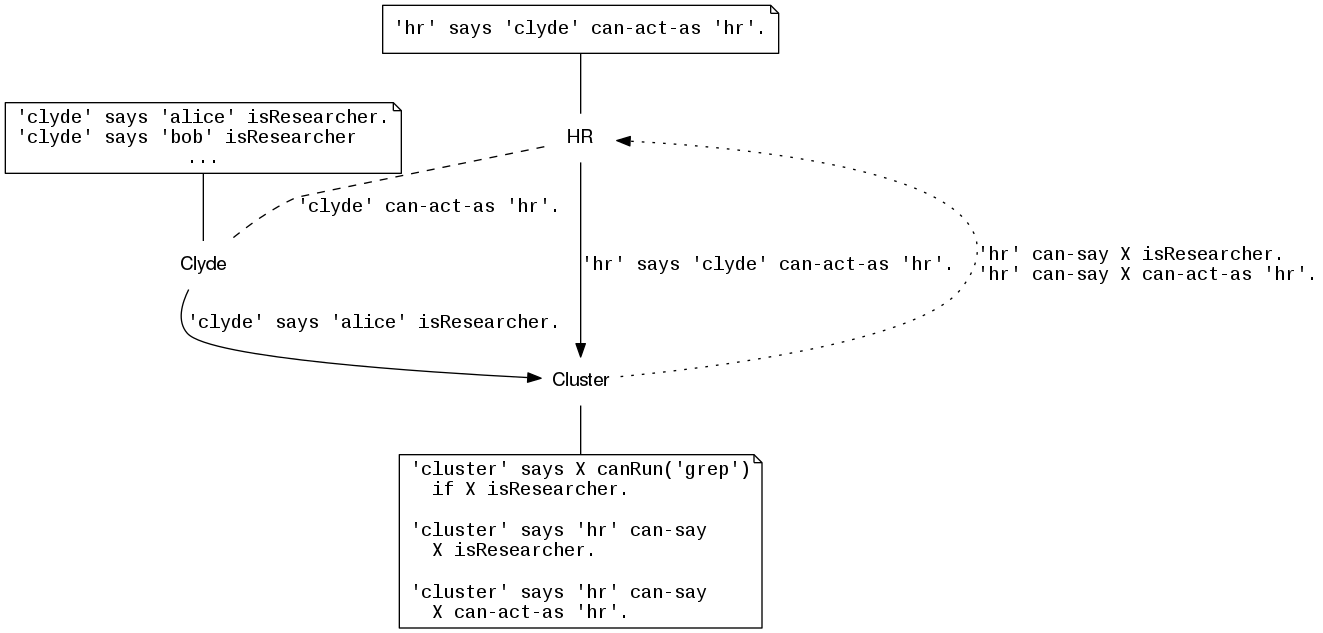
\includegraphics[width=\textwidth]{figures/secpal-example-roles.png}
  \caption[Example of delegation with roles.]{Example of delegation with roles.  Role relationships are shown with dashed links.}
  \label{fig:roles-example}
\end{figure}

An alternative to the delegation to the HR server to determine if
Alice was a researcher would be to use delegation with roles (shown in
\autoref{fig:roles-example}).  HR may consist of many principals.  The
cluster may be happy to accept the word of anyone who works in HR as
if they were HR.  To do this the cluster adds a delegation to HR that
they can name anyone who acts as them, and HR respond by saying that
Clyde can act for them.
\begin{lstlisting}
'cluster' says 'hr' can-say
  X can-act-as 'hr'.
'hr' says 'clyde' can-act-as 'hr'.
\end{lstlisting}
Now on the cluster Clyde's word is as good as HR's.
Clyde sends the necessary facts about Alice and the program can be run as before.
It is important to note that any restrictions on HR also apply to Clyde.  He still cannot delegate the decision further.

\begin{figure}
  \centering
  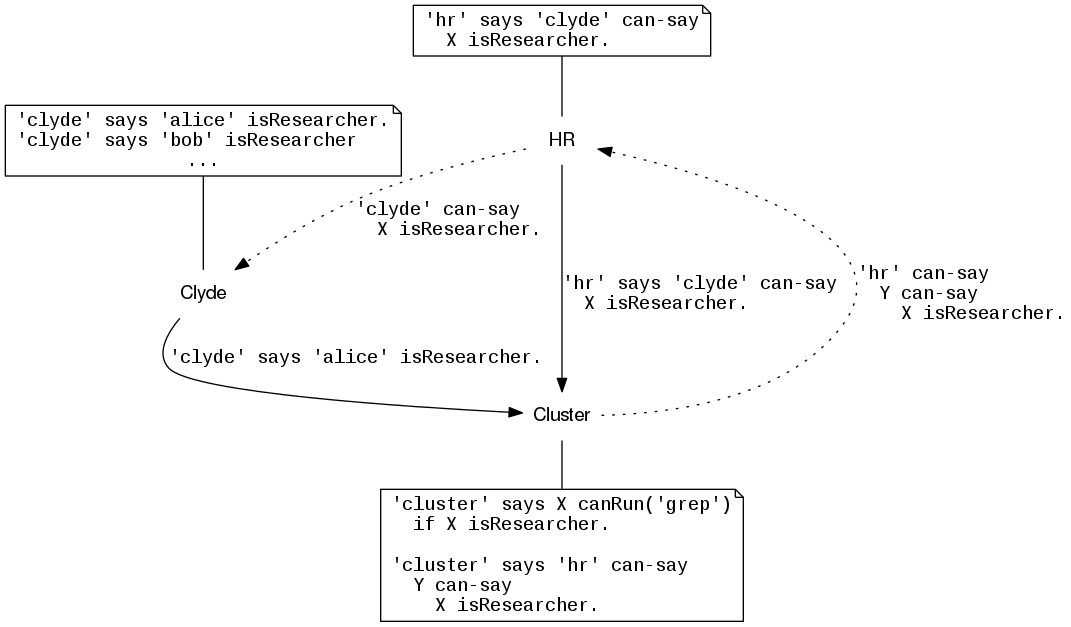
\includegraphics[width=\textwidth]{figures/secpal-example-delegation2.png}
  \caption{Example of depth bounded delegation.}
  \label{fig:depth-example}
\end{figure}

As an alternative to roles, depth-bounded delegation with the
\emph{can-say} statement could also have been used
(\autoref{fig:depth-example}).  In this case instead of delegating the
decision of who is a researcher to HR, the cluster delegates the
\emph{decision of who can make the decision} to HR.  HR makes the
delegation to Clyde, and the process continues as before.
Depth-bounded delegation allows delegation statements to be chained to
an arbitrary (but finite) depth, without allowing for unbounded
delegation.  It is often preferable to roles as it allows HR to
delegate some but not all decisions to others.  If the role assignment
is used then, on the cluster, anywhere \texttt{'hr'} follows the
\texttt{says} in an assertion, then it can be replaced with
\texttt{'clyde'}: making them effectively equivalent.

SecPAL's delegation mechanisms can describe a large number of
different relationships, whilst remaining conceptually and
semantically extremely simple.  This power makes SecPAL an exteremely
attractive authorization language for situations where entities are
distributed and there is no central decision maker: whatever
relationship each of the entities have SecPAL can describe it.

\end{document}

%%% Local Variables:
%%% mode: latex
%%% TeX-master: "../ch2"
%%% End:
